\subsection{Loads}
The loads acting on the footings are shown in \S \ref{sc_column_internal_forces}.

\subsection{Load combinations}
The load combinations are shown in tables \ref{ULS} and \ref{SLS}.

\subsection{Footing dimensions and reinforcement}
The dimensions and the reinforcement of the footings are indicated in the table \ref{tb_column_footing_schedule}. The position of the footing in the building grid is indicated at the last column.

\begin{table}
  \begin{center}
    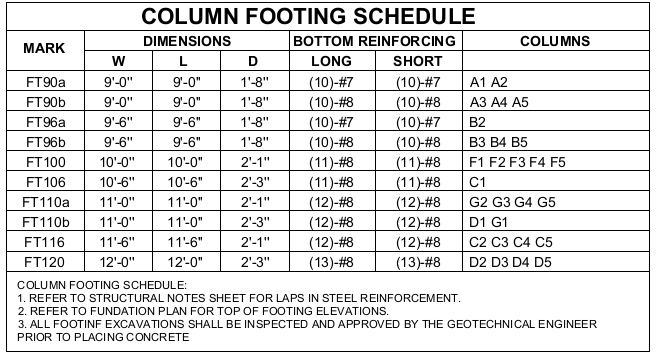
\includegraphics[width=90mm]{figures/column_footing_schedule.png}
  \end{center}
    \caption{Column footing schedule.}\label{tb_column_footing_schedule}
\end{table}

\subsection{Limit state checking}
\subsubsection{Allowable soil-bearing pressures}
The results obtained for the verification of the soil-bearing capacity are shown in the table \ref{tb_soil_bearing}.

\begin{table}
\begin{center}
  \begin{scriptsize}
  \begin{tabular}{|l|l|r|r|}
\hline
Foundation & Worst & Vertical & Capacity\\
 & combination & load (kN) & factor\\
\hline
 A1 &  SLS04\_a & -356.20 & 0.33\\
 A2 &  SLS02\_a & -644.78 & 0.60\\
 A3 &  SLS02\_a & -950.92 & 0.88\\
 A4 &  SLS02\_a & -881.82 & 0.82\\
 A5 &  SLS04\_b & -933.03 & 0.86\\
 B2 &  SLS02\_a & -670.79 & 0.56\\
 B3 &  SLS02\_a & -1,030.65 & 0.86\\
 B4 &  SLS02\_a & -968.24 & 0.80\\
 B5 &  SLS04\_b & -972.32 & 0.81\\
 C1 &  SLS02\_a & -1,460.67 & 0.99\\
 C2 &  SLS02\_a & -1,742.45 & 0.99\\
 C3 &  SLS02\_a & -1,750.31 & 0.99\\
 C4 &  SLS02\_a & -1,751.62 & 0.99\\
 C5 &  SLS02\_a & -1,660.02 & 0.94\\
 D1 &  SLS02\_a & -1,648.12 & 1.02\\
 D2 &  SLS04\_a & -1,950.01 & 1.01\\
 D3 &  SLS04\_a & -1,959.12 & 1.02\\
 D4 &  SLS04\_a & -1,960.14 & 1.02\\
 D5 &  SLS04\_a & -1,838.69 & 0.96\\
 F1 &  SLS02\_a & -1,090.88 & 0.82\\
 F2 &  SLS02\_a & -997.32 & 0.75\\
 F3 &  SLS02\_a & -1,011.87 & 0.76\\
 F4 &  SLS02\_a & -1,005.30 & 0.75\\
 F5 &  SLS04\_b & -741.90 & 0.56\\
 G1 &  SLS02\_a & -1,496.86 & 0.93\\
 G2 &  SLS02\_a & -1,256.06 & 0.78\\
 G3 &  SLS02\_a & -1,227.94 & 0.76\\
 G4 &  SLS02\_a & -1,137.75 & 0.70\\
 G5 &  SLS04\_b & -1,167.26 & 0.72\\
\hline
  \end{tabular}
  \end{scriptsize}
  \end{center}
\caption{Soil bearing pressures. Capacity factors}\label{tb_soil_bearing}
\end{table}

\subsubsection{Flexure design}
The capacity factor for the bending in the longitudinal and transverse directions are shown in figures \ref{fg_flexure_design_cf_long_direction} and \ref{fg_flexure_design_cf_transv_direction}.

\subsubsection{Shear design}
The results of the shear strength verification are shown in the table \ref{tb_footings_shear_design}. The results of the punching shear strength verification are shown in table \ref{tb_footings_puching_design}.

\begin{table}
\begin{center}
  \begin{scriptsize}
\begin{tabular}{|l|l|r|r|r|r|r|r|r|r|}
\hline
Footing & Worst & Vertical & thickness & l & d & c & Vd/l & Vu & CF\\
 & combination & load (kN) & (m) & (m) & (m) & (m) & kN/m & kN/m & \\
\hline
 A1 &  SLS04\_a & -356.20 & 0.51 & 2.74 & 0.46 & 0.41 & 33.66 & 280.00 & 0.12\\
 A2 &  SLS02\_a & -644.78 & 0.51 & 2.74 & 0.46 & 0.41 & 60.94 & 280.00 & 0.22\\
 A3 &  SLS02\_a & -950.92 & 0.51 & 2.74 & 0.46 & 0.41 & 89.87 & 280.00 & 0.32\\
 A4 &  SLS02\_a & -881.82 & 0.51 & 2.74 & 0.46 & 0.41 & 83.34 & 280.00 & 0.30\\
 A5 &  SLS04\_b & -933.03 & 0.51 & 2.74 & 0.46 & 0.41 & 88.18 & 280.00 & 0.31\\
 B2 &  SLS02\_a & -670.79 & 0.51 & 2.90 & 0.46 & 0.41 & 63.00 & 280.00 & 0.22\\
 B3 &  SLS02\_a & -1,030.65 & 0.51 & 2.90 & 0.46 & 0.41 & 96.79 & 280.00 & 0.35\\
 B4 &  SLS02\_a & -968.24 & 0.51 & 2.90 & 0.46 & 0.41 & 90.93 & 280.00 & 0.32\\
 B5 &  SLS04\_b & -972.32 & 0.51 & 2.90 & 0.46 & 0.41 & 91.31 & 280.00 & 0.33\\
 C1 &  SLS02\_a & -1,460.67 & 0.69 & 3.20 & 0.62 & 0.41 & 111.20 & 378.00 & 0.29\\
 C2 &  SLS02\_a & -1,742.45 & 0.64 & 3.51 & 0.57 & 0.41 & 138.68 & 350.00 & 0.40\\
 C3 &  SLS02\_a & -1,750.31 & 0.64 & 3.51 & 0.57 & 0.41 & 139.31 & 350.00 & 0.40\\
 C4 &  SLS02\_a & -1,751.62 & 0.64 & 3.51 & 0.57 & 0.41 & 139.42 & 350.00 & 0.40\\
 C5 &  SLS02\_a & -1,660.02 & 0.64 & 3.51 & 0.57 & 0.41 & 132.12 & 350.00 & 0.38\\
 D1 &  SLS02\_a & -1,648.12 & 0.69 & 3.35 & 0.62 & 0.41 & 125.50 & 378.00 & 0.33\\
 D2 &  SLS04\_a & -1,950.01 & 0.64 & 3.66 & 0.57 & 0.41 & 153.65 & 350.00 & 0.44\\
 D3 &  SLS04\_a & -1,959.12 & 0.64 & 3.66 & 0.57 & 0.41 & 154.37 & 350.00 & 0.44\\
 D4 &  SLS04\_a & -1,960.14 & 0.64 & 3.66 & 0.57 & 0.41 & 154.45 & 350.00 & 0.44\\
 D5 &  SLS04\_a & -1,838.69 & 0.64 & 3.66 & 0.57 & 0.41 & 144.88 & 350.00 & 0.41\\
 F1 &  SLS02\_a & -1,090.88 & 0.64 & 3.05 & 0.57 & 0.41 & 87.98 & 350.00 & 0.25\\
 F2 &  SLS02\_a & -997.32 & 0.64 & 3.05 & 0.57 & 0.41 & 80.44 & 350.00 & 0.23\\
 F3 &  SLS02\_a & -1,011.87 & 0.64 & 3.05 & 0.57 & 0.41 & 81.61 & 350.00 & 0.23\\
 F4 &  SLS02\_a & -1,005.30 & 0.64 & 3.05 & 0.57 & 0.41 & 81.08 & 350.00 & 0.23\\
 F5 &  SLS04\_b & -741.90 & 0.64 & 3.05 & 0.57 & 0.41 & 59.84 & 350.00 & 0.17\\
 G1 &  SLS02\_a & -1,496.86 & 0.69 & 3.35 & 0.62 & 0.41 & 113.98 & 378.00 & 0.30\\
 G2 &  SLS02\_a & -1,256.06 & 0.64 & 3.35 & 0.57 & 0.41 & 100.75 & 350.00 & 0.29\\
 G3 &  SLS02\_a & -1,227.94 & 0.64 & 3.35 & 0.57 & 0.41 & 98.50 & 350.00 & 0.28\\
 G4 &  SLS02\_a & -1,137.75 & 0.64 & 3.35 & 0.57 & 0.41 & 91.26 & 350.00 & 0.26\\
 G5 &  SLS04\_b & -1,167.26 & 0.64 & 3.35 & 0.57 & 0.41 & 93.63 & 350.00 & 0.27\\
\hline
  \end{tabular}
  \end{scriptsize}
\end{center}
\caption{Shear design. Capacity factors}\label{tb_footings_shear_design}
\end{table}


\begin{table}
\begin{center}
  \begin{scriptsize}
  \begin{tabular}{|l|l|r|r|r|r|r|r|r|r|}
\hline
Footing & Worst & Vertical & thickness & L & d & c & Vd/l & Vu & CF\\
 & combination & load (kN) & (m) & (m) & (m) & (m) & kN/m & kN/m & \\
\hline
 A1 &  SLS04\_a & -356.20 & 0.51 & 2.74 & 0.46 & 0.41 & 92.90 & 517.97 & 0.18\\
 A2 &  SLS02\_a & -644.78 & 0.51 & 2.74 & 0.46 & 0.41 & 168.16 & 517.97 & 0.32\\
 A3 &  SLS02\_a & -950.92 & 0.51 & 2.74 & 0.46 & 0.41 & 248.00 & 517.97 & 0.48\\
 A4 &  SLS02\_a & -881.82 & 0.51 & 2.74 & 0.46 & 0.41 & 229.98 & 517.97 & 0.44\\
 A5 &  SLS04\_b & -933.03 & 0.51 & 2.74 & 0.46 & 0.41 & 243.33 & 517.97 & 0.47\\
 B1 &  SLS02\_a & -429.53 & 0.51 & 2.90 & 0.46 & 0.41 & 113.28 & 517.97 & 0.22\\
 B2 &  SLS02\_a & -670.79 & 0.51 & 2.90 & 0.46 & 0.41 & 176.91 & 517.97 & 0.34\\
 B3 &  SLS02\_a & -1,030.65 & 0.51 & 2.90 & 0.46 & 0.41 & 271.82 & 517.97 & 0.52\\
 B4 &  SLS02\_a & -968.24 & 0.51 & 2.90 & 0.46 & 0.41 & 255.36 & 517.97 & 0.49\\
 B5 &  SLS04\_b & -972.32 & 0.51 & 2.90 & 0.46 & 0.41 & 256.43 & 517.97 & 0.50\\
 C1 &  SLS02\_a & -1,460.67 & 0.69 & 3.20 & 0.62 & 0.41 & 320.25 & 699.26 & 0.46\\
 C2 &  SLS02\_a & -1,742.45 & 0.64 & 3.51 & 0.57 & 0.41 & 410.79 & 647.47 & 0.63\\
 C3 &  SLS02\_a & -1,750.31 & 0.64 & 3.51 & 0.57 & 0.41 & 412.64 & 647.47 & 0.64\\
 C4 &  SLS02\_a & -1,751.62 & 0.64 & 3.51 & 0.57 & 0.41 & 412.95 & 647.47 & 0.64\\
 C5 &  SLS02\_a & -1,660.02 & 0.64 & 3.51 & 0.57 & 0.41 & 391.35 & 647.47 & 0.60\\
 D1 &  SLS02\_a & -1,648.12 & 0.69 & 3.35 & 0.62 & 0.41 & 365.00 & 699.26 & 0.52\\
 D2 &  SLS04\_a & -1,950.01 & 0.64 & 3.66 & 0.57 & 0.41 & 462.88 & 647.47 & 0.71\\
 D3 &  SLS04\_a & -1,959.12 & 0.64 & 3.66 & 0.57 & 0.41 & 465.05 & 647.47 & 0.72\\
 D4 &  SLS04\_a & -1,960.14 & 0.64 & 3.66 & 0.57 & 0.41 & 465.29 & 647.47 & 0.72\\
 D5 &  SLS04\_a & -1,838.69 & 0.64 & 3.66 & 0.57 & 0.41 & 436.46 & 647.47 & 0.67\\
 F1 &  SLS02\_a & -1,090.88 & 0.64 & 3.05 & 0.57 & 0.41 & 250.18 & 647.47 & 0.39\\
 F2 &  SLS02\_a & -997.32 & 0.64 & 3.05 & 0.57 & 0.41 & 228.72 & 647.47 & 0.35\\
 F3 &  SLS02\_a & -1,011.87 & 0.64 & 3.05 & 0.57 & 0.41 & 232.06 & 647.47 & 0.36\\
 F4 &  SLS02\_a & -1,005.30 & 0.64 & 3.05 & 0.57 & 0.41 & 230.55 & 647.47 & 0.36\\
 F5 &  SLS04\_b & -741.90 & 0.64 & 3.05 & 0.57 & 0.41 & 170.14 & 647.47 & 0.26\\
 G1 &  SLS02\_a & -1,496.86 & 0.69 & 3.35 & 0.62 & 0.41 & 331.50 & 699.26 & 0.47\\
 G2 &  SLS02\_a & -1,256.06 & 0.64 & 3.35 & 0.57 & 0.41 & 293.79 & 647.47 & 0.45\\
 G3 &  SLS02\_a & -1,227.94 & 0.64 & 3.35 & 0.57 & 0.41 & 287.22 & 647.47 & 0.44\\
 G4 &  SLS02\_a & -1,137.75 & 0.64 & 3.35 & 0.57 & 0.41 & 266.12 & 647.47 & 0.41\\
 G5 &  SLS04\_b & -1,167.26 & 0.64 & 3.35 & 0.57 & 0.41 & 273.02 & 647.47 & 0.42\\
\hline
  \end{tabular}
  \end{scriptsize}
  \end{center}
\caption{Two-way shear design. Capacity factors}\label{tb_footings_puching_design}
\end{table}

\begin{figure}
  \begin{center}
    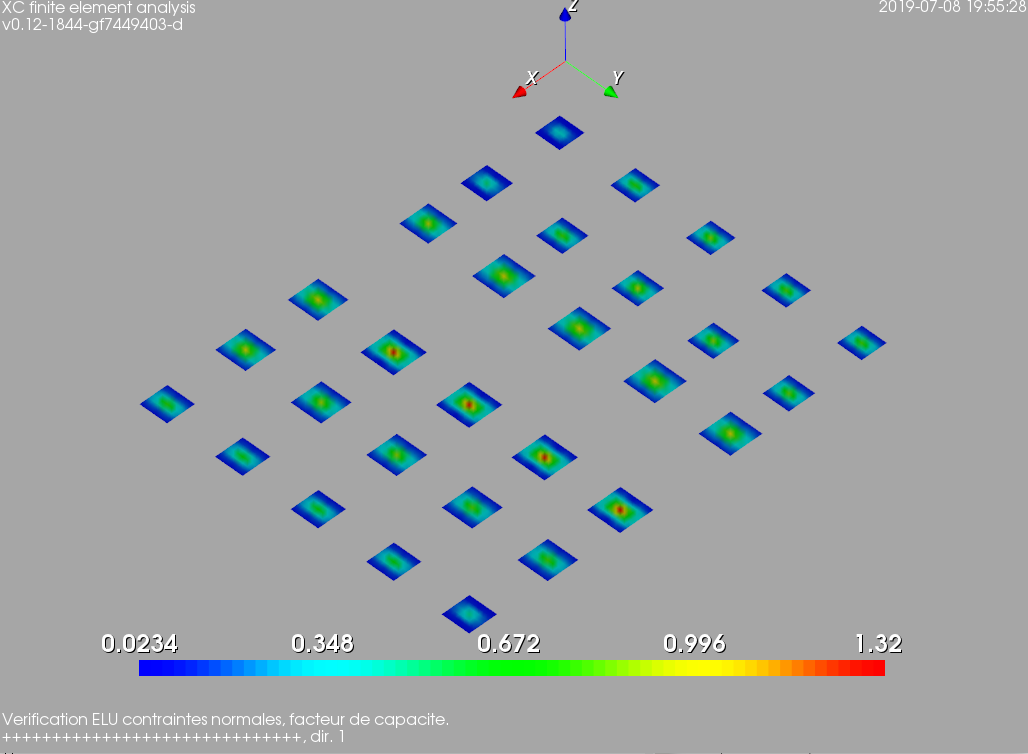
\includegraphics[width=90mm]{figures/flexure_design_cf_long_direction}
  \end{center}
    \caption{Flexure in the longitudinal direction. Capacity factor.}\label{fg_flexure_design_cf_long_direction}
\end{figure}

\begin{figure}
  \begin{center}
    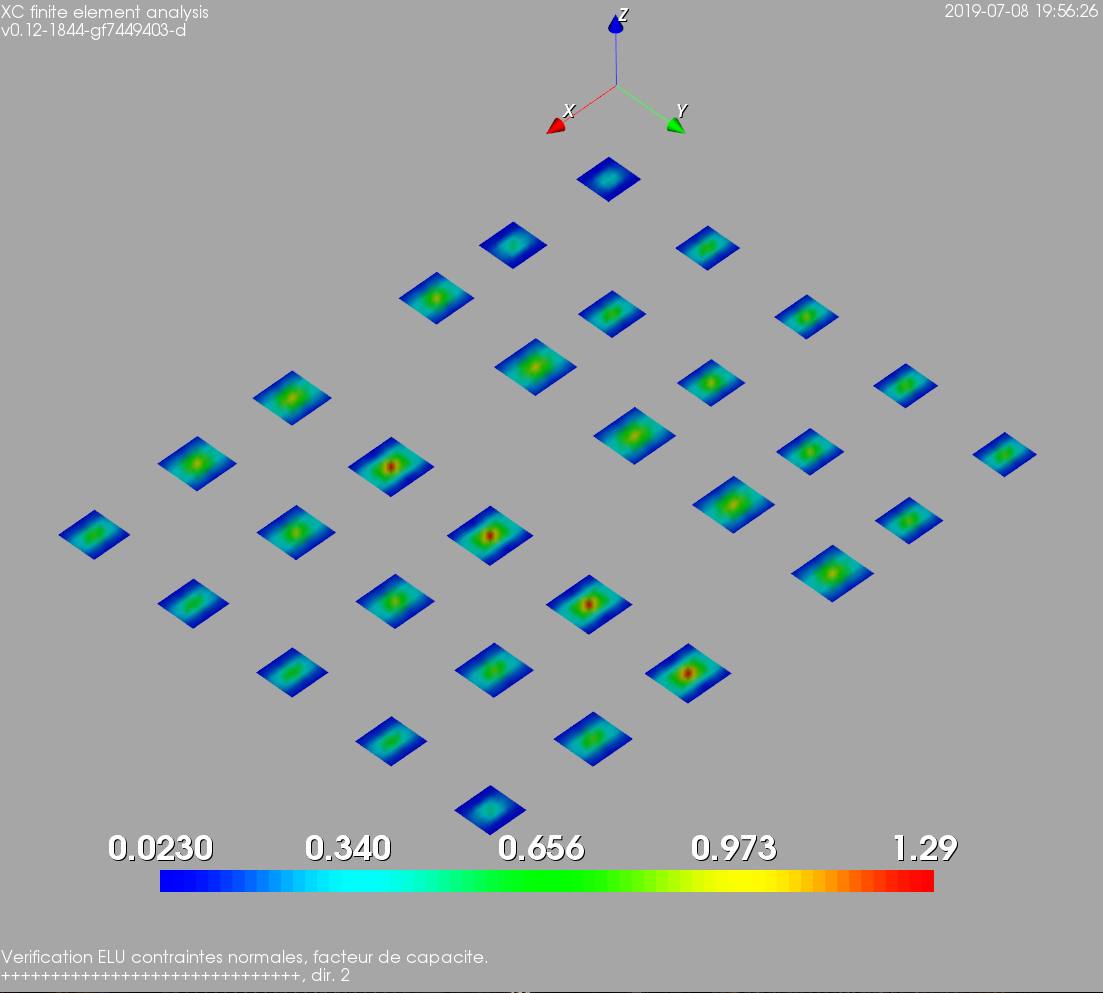
\includegraphics[width=90mm]{figures/flexure_design_cf_transv_direction}
  \end{center}
    \caption{Flexure in the transverse direction. Capacity factor.}\label{fg_flexure_design_cf_transv_direction}
\end{figure}

%%  LocalWords:  kN Flexure Vd Vu
